% Chapter 3
\chapter{Resultados}\label{chap:Results}

Neste capítulo são apresentados os resultados do trabalho desenvolvido,
apresentando a criação do repositório institucional proposto, desde a
sua concepção, \emph{backlog} do produto, protótipos, resultado final
e validação das hipóteses.

\section{Concepção do Repositório Institucional}

A concepção do repositório institucional proposto foi realizada com base
nos desafios e problemas relatados nos trabalhos relacionados, e na análise
dos pontos positivos e negativos encontrados em outros sistemas de repositório
institucional existentes.

Como um dos principais diferenciais do repositório proposto, é que desde o
inicio de seu desenvolvimento ele foi projetado para ser facilmente implantado
e executado em ambientes baseados em nuvem, sendo assim todas as suas configurações
podem ser realizadas por meio de variáveis de ambiente, que em geral podem ser
facilmente definidas pelo próprio painel ou \emph{dashboard} fornecido pelo
provedor de nuvem. A ideia é nunca precisar acessar remotamente a máquina
em que a aplicação está sendo executada para realizar qualquer tipo de configuração.

Outro ponto de diferença é que o repositório proposto somente aceita arquivos no
formato PDF, visando mitigar problemas relacionados a formatação do documento, e
buscando garantir que o usuário ao acessar as publicações, visualize
o documento da mesma forma que o autor originalmente a escreveu. Esta redução
do escopo de formatos de arquivos aceitos pelo repositório, também garante que
todas as publicações estejam normalizadas em um mesmo formato, permitindo a
utilização de técnicas mais especializadas para a extração de texto dos documentos.

Para realizar a escolha do nome e identidade visual do repositório, foram buscados
por termos que remetessem a "Repositório", "Acesso Aberto'' e "Pesquisa", chegando
a escolha do nome RESOAR, uma sigla em inglês para \emph{Research Open Access Repository}.
A sigla "OAR'' que remete a \emph{Open Access Repository} já é baste difundida, e
pode ser encontrada em nomes como o OpenDOAR\footnote{https://v2.sherpa.ac.uk/opendoar/} e
ROARMAP\footnote{https://roarmap.eprints.org/}.

\begin{figure}[H]
    \caption{Identidade visual do repositório}
    \centering
    \frame{
\includegraphics[scale=0.0558]{img/resoar.png}}
    \label{fig:resoar}
    \source{Do próprio autor}
\end{figure}

A Figura \ref{fig:resoar} apresenta a logo ou identidade visual do repositório,
que foi elaborada por um designer contratado da região de Três de Maio - RS,
que desenvolveu tanto a identidade visual quanto os primeiros protótipos do repositório.

Em sua composição é possível perceber um simbolo de lupa embutido na primeira letra "R''
representando a pesquisa. A cor padrão da logo foi escolhida como o laranja com
o código HEX \#ff5400, porém o simbolo também pode ser exibido em outras variações,
como em preto e branco, escala de cinza ou outras cores.

\section{Backlog do produto}

Nesta seção será apresentado o \emph{backlog} do produto que foi desenvolvido
seguindo a metodologia de \emph{User Stories}, contendo uma lista de funcionalidades
que o sistema final deve conter, além de \emph{mockups} das telas, servindo como uma
base para o desenvolvimento da aplicação.

\begin{table}[H]
    \caption{Tela de Login}
    \begin{tabular}{|p{1cm}|p{14cm}|}
        \hline
        \multicolumn{1}{|c|}{\textbf{01}} & \textbf{Tela de Login}                                                                                                                                                                                                                                                                        \\ \hline
        \multicolumn{2}{|l|}{\begin{tabular}[c]{@{}l@{}}\textbf{Como} usuário do sistema\\ \textbf{Eu quero} realizar o login utilizando meu email e senha\\ \textbf{Para que} possa utilizar as funções presentes no sistema.\end{tabular}}                                                                                              \\ \hline
        \multicolumn{2}{|l|}{\textbf{Critérios de aceitação}}                                                                                                                                                                                                                                                                             \\ \hline
        \multicolumn{2}{|l|}{\begin{tabular}[c]{@{}l@{}}1. Deve possui o botão de exibir/esconder a senha.\\2. Deve possuir os atalhos para as telas de recuperação de senha e cadastro\\ de usuário.\\3. Caso o usuário digitar a senha incorretamente mais de 3 vezes, deve solicitar\\ a solução de um desafio captcha. \end{tabular}} \\ \hline
        \multicolumn{2}{|c|}{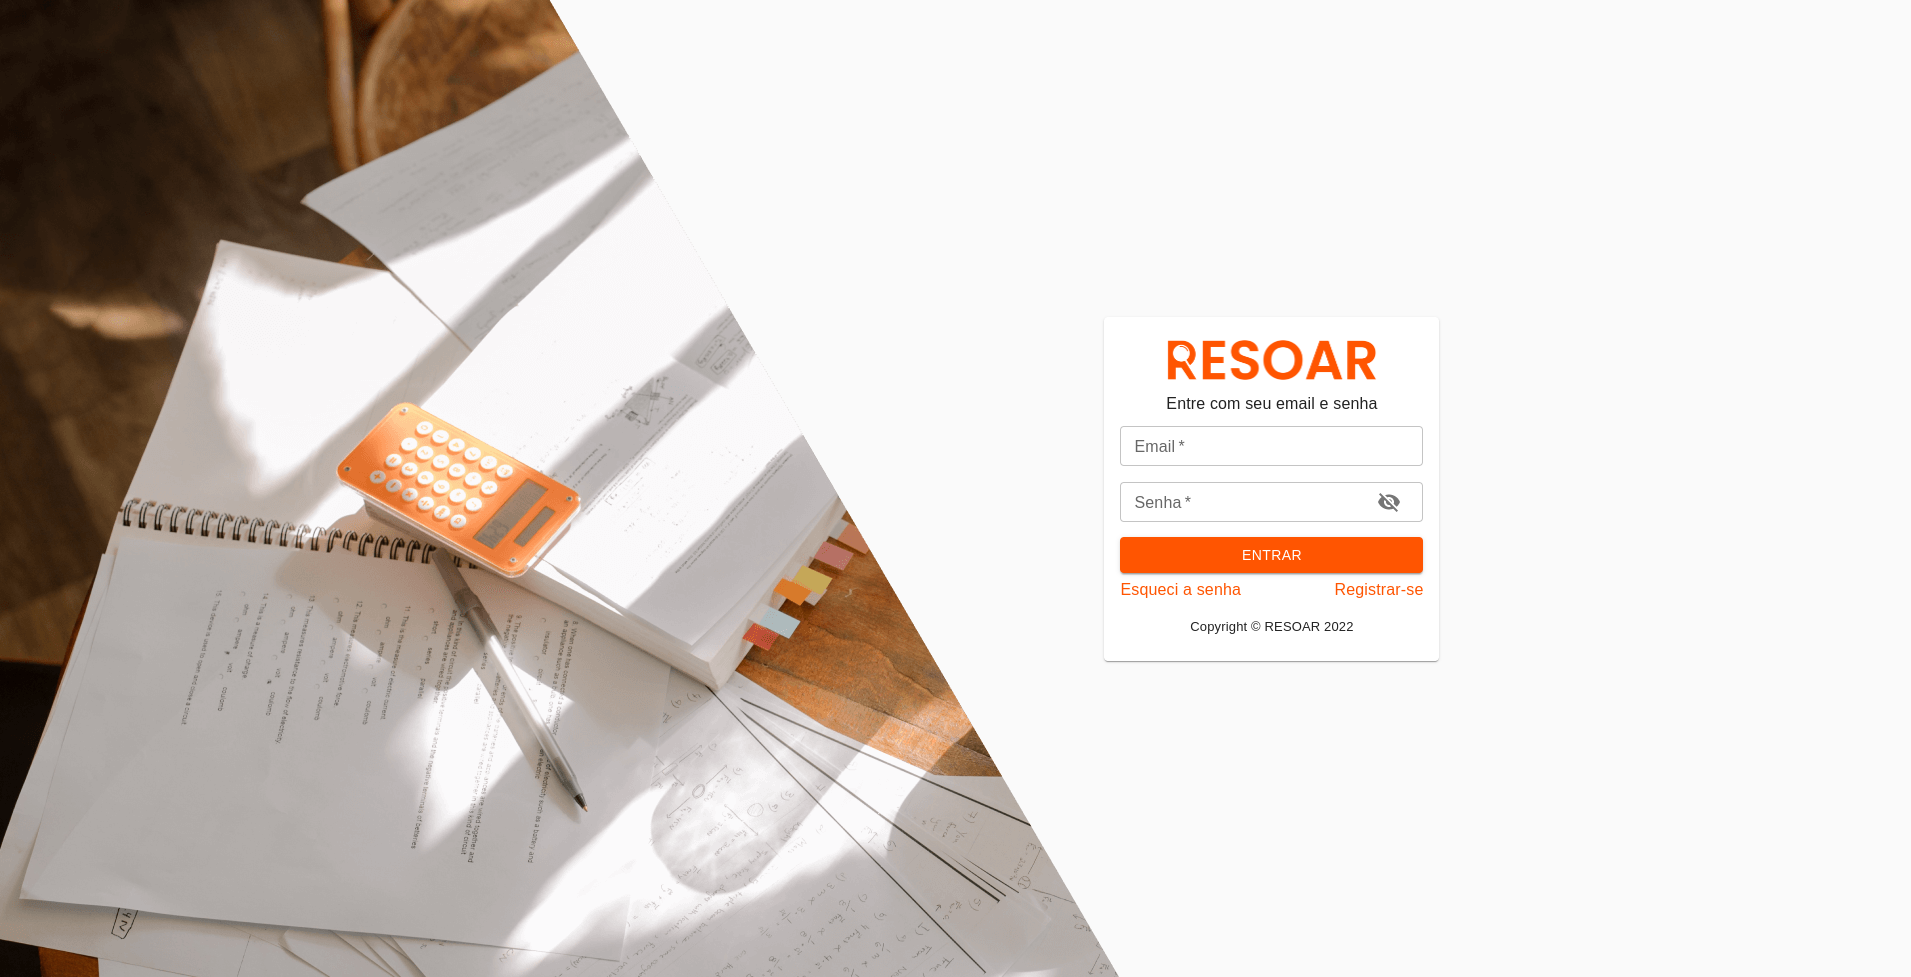
\includegraphics[scale=0.296]{img/resoar-login.png}}                                                                                                                                                                                                                                                         \\ \hline
    \end{tabular}
\end{table}

\begin{table}[H]
    \caption{Cadastro de usuário}
    \begin{tabular}{|p{1cm}|p{14cm}|}
        \hline
        \multicolumn{1}{|c|}{\textbf{02}} & \textbf{Cadastro de usuário}                                                                                                                                                                                 \\ \hline
        \multicolumn{2}{|l|}{\begin{tabular}[c]{@{}l@{}}\textbf{Como} novo usuário\\ \textbf{Eu quero} me cadastrar no sistema\\ \textbf{Para que} possa entrar no sistema.\end{tabular}}                                                                \\ \hline
        \multicolumn{2}{|l|}{\textbf{Critérios de aceitação}}                                                                                                                                                                                            \\ \hline
        \multicolumn{2}{|l|}{\begin{tabular}[c]{@{}l@{}}1. Deve validar se já existe um usuário cadastrado com o mesmo email.\\2. Deve validar se os dois campos de senha são iguais.\\3. Deve solicitar a solução de um desafio captcha. \end{tabular}} \\ \hline
        \multicolumn{2}{|c|}{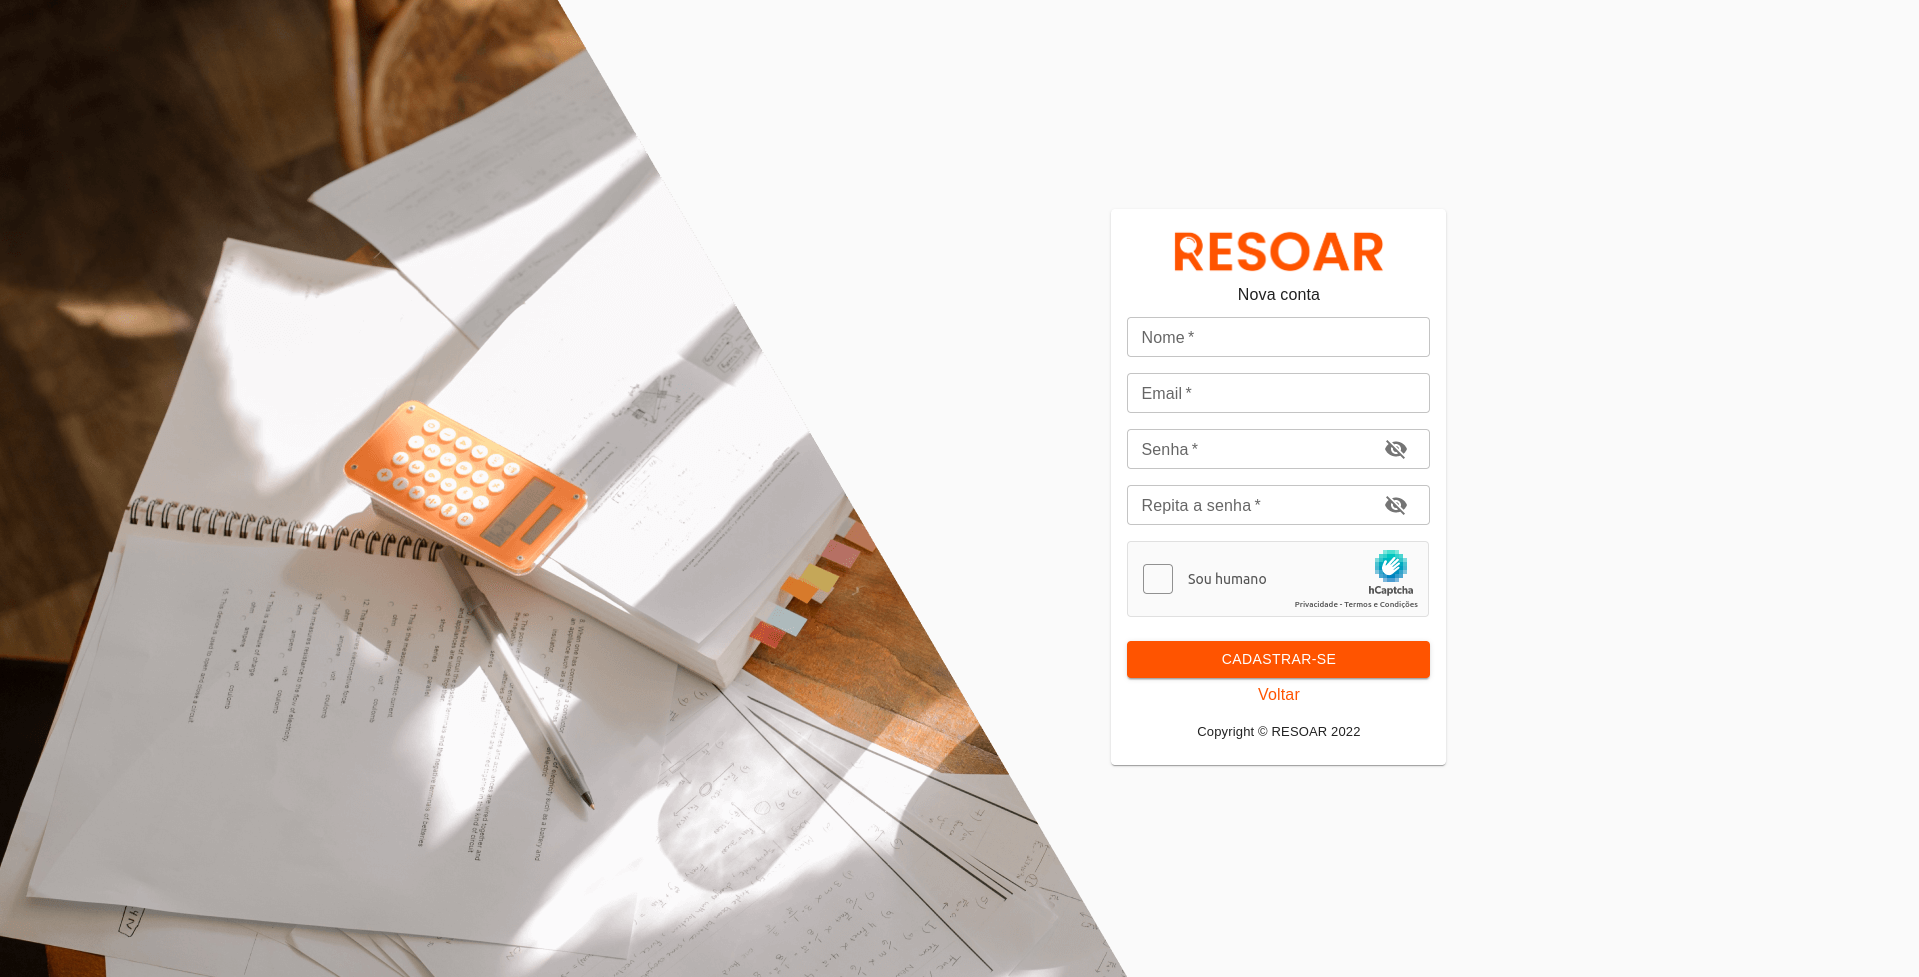
\includegraphics[scale=0.294]{img/resoar-new-account.png}}                                                                                                                                                                  \\ \hline
    \end{tabular}
\end{table}

\begin{table}[H]
    \caption{Recuperação de senha}
    \begin{tabular}{|p{1cm}|p{14cm}|}
        \hline
        \multicolumn{1}{|c|}{\textbf{03}} & \textbf{Recuperação de senha}                                                                                                                                                                                   \\ \hline
        \multicolumn{2}{|l|}{\begin{tabular}[c]{@{}l@{}}\textbf{Como} usuário do sistema\\ \textbf{Eu quero} poder solicitar um email de recuperação de senha\\ \textbf{Para que} possa criar uma nova senha para meu usuário.\end{tabular}}                \\ \hline
        \multicolumn{2}{|l|}{\textbf{Critérios de aceitação}}                                                                                                                                                                                               \\ \hline
        \multicolumn{2}{|l|}{\begin{tabular}[c]{@{}l@{}}1. Deve validar se o email informado existe no sistema.\\2. Deve enviar um email de recuperação, com validade máxima de 3 horas.\\3. Deve solicitar a solução de um desafio captcha. \end{tabular}} \\ \hline
        \multicolumn{2}{|c|}{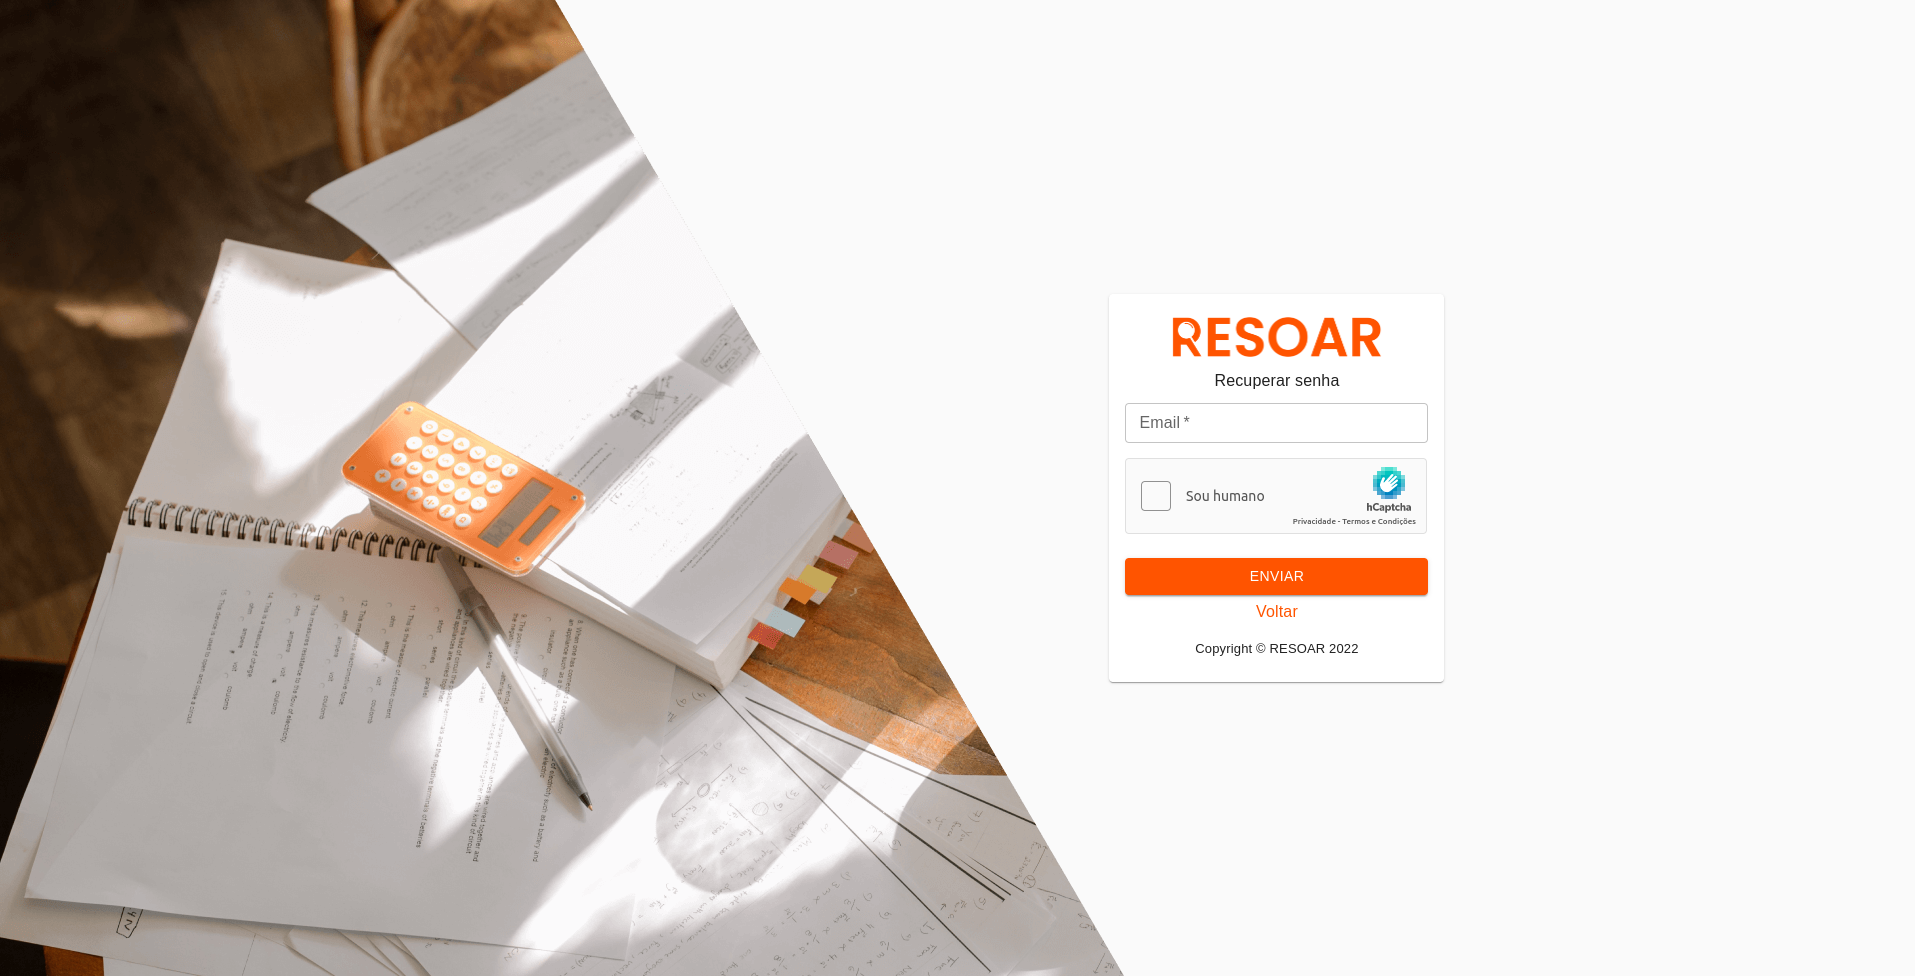
\includegraphics[scale=0.294]{img/resoar-password-recovery.png}}                                                                                                                                                               \\ \hline
    \end{tabular}
\end{table}

\begin{table}[H]
    \caption{Visão geral}
    \begin{tabular}{|p{1cm}|p{14cm}|}
        \hline
        \multicolumn{1}{|c|}{\textbf{04}} & \textbf{Visão geral}                                                                                                                                                                                                                                                                            \\ \hline
        \multicolumn{2}{|l|}{\begin{tabular}[c]{@{}l@{}}\textbf{Como} usuário do sistema\\ \textbf{Eu quero} acessar uma tela de boas vindas ao entrar no sistema, contendo as\\ minhas publicações mais recentes, publicações salvas, e histórico de\\ publicações acessadas.\\ \textbf{Para que} tenha um ponto de partida.\end{tabular}} \\ \hline
        \multicolumn{2}{|l|}{\textbf{Critérios de aceitação}}                                                                                                                                                                                                                                                                               \\ \hline
        \multicolumn{2}{|l|}{\begin{tabular}[c]{@{}l@{}}1. Deve exibir ao menos as 3 últimas publicações do usuário.\\2. Deve exibir ao menos as 3 últimas publicações salvas para leitura. \end{tabular}}                                                                                                                                  \\ \hline
        \multicolumn{2}{|c|}{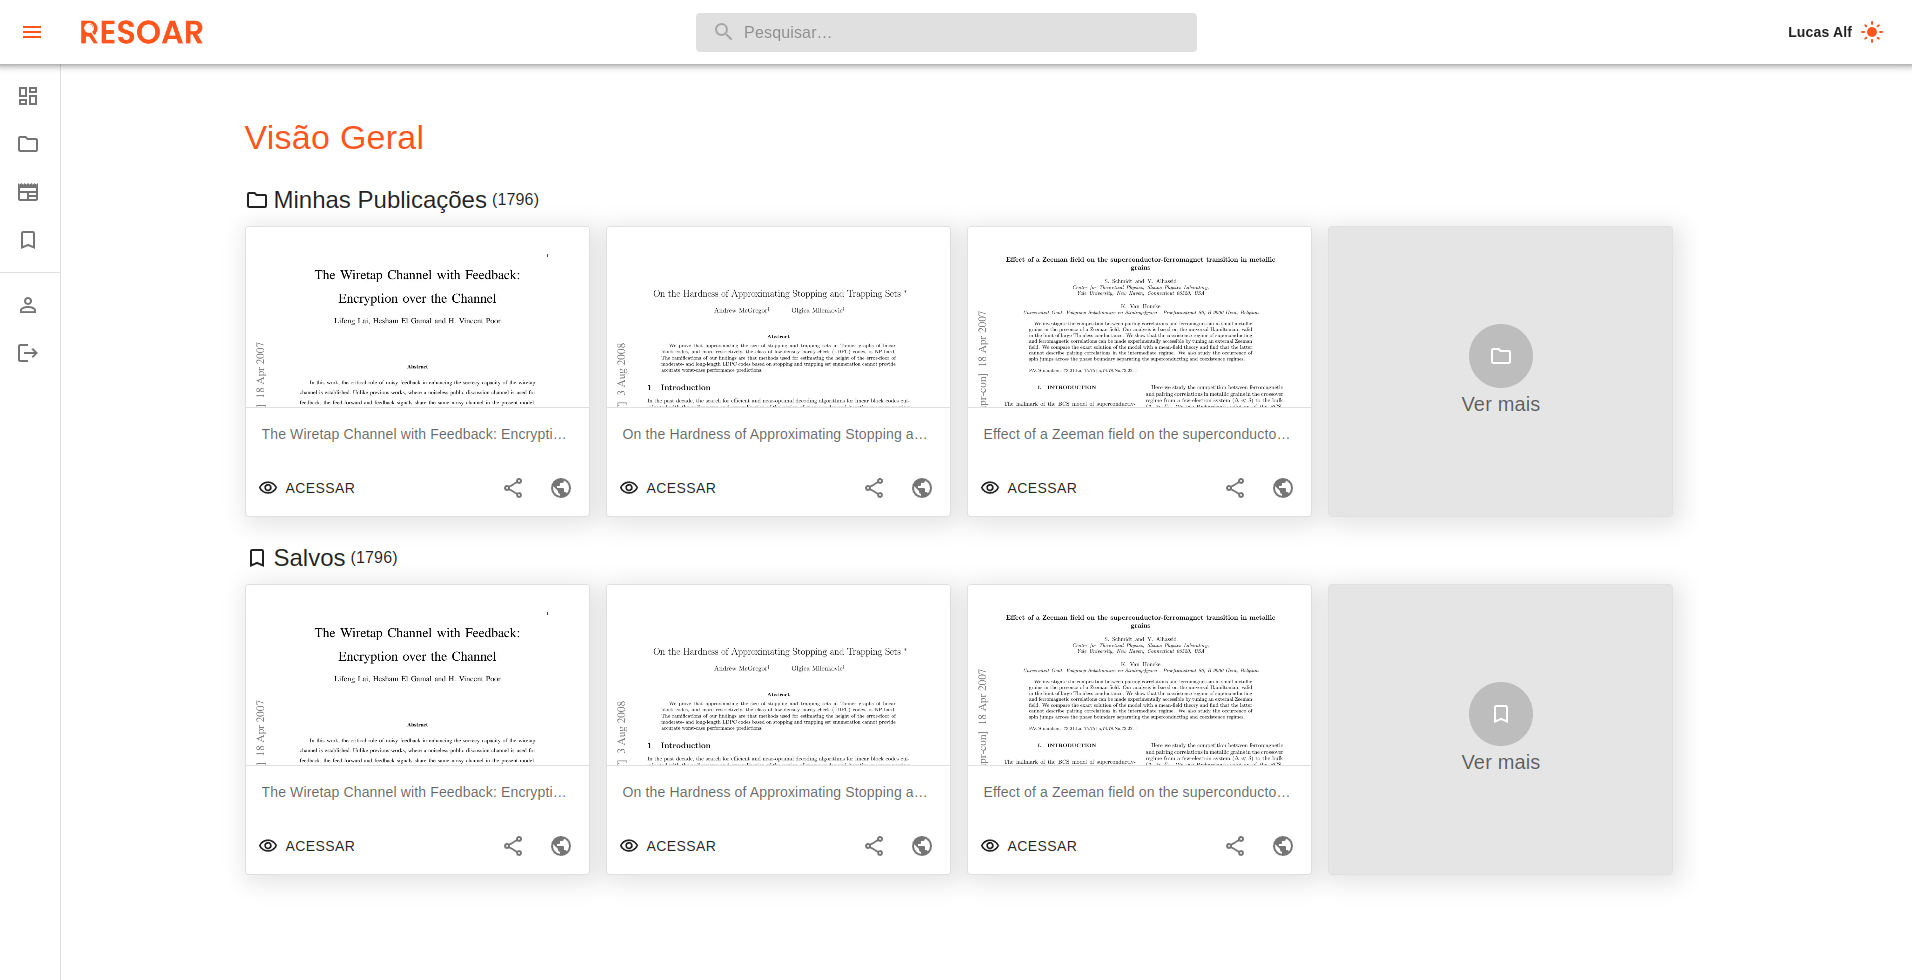
\includegraphics[scale=0.294]{img/resoar-overview.png}}                                                                                                                                                                                                                                                        \\ \hline
    \end{tabular}
\end{table}

\begin{table}[H]
    \caption{Minhas publicações}
    \begin{tabular}{|p{1cm}|p{14cm}|}
        \hline
        \multicolumn{1}{|c|}{\textbf{05}} & \textbf{Minhas publicações}                                                                                                                                                                                                                                                                                                                             \\ \hline
        \multicolumn{2}{|l|}{\begin{tabular}[c]{@{}l@{}}\textbf{Como} usuário do sistema\\ \textbf{Eu quero} acessar uma listagem contendo todas as minhas publicações\\ \textbf{Para que} possa navegar pelas publicações que realizei.\end{tabular}}                                                                                                                                              \\ \hline
        \multicolumn{2}{|l|}{\textbf{Critérios de aceitação}}                                                                                                                                                                                                                                                                                                                                       \\ \hline
        \multicolumn{2}{|l|}{\begin{tabular}[c]{@{}l@{}}1. Deve permitir a filtragem de publicações pelo título.\\2. Deve exibir na listagem o título, a imagem de capa, os autores, orientadores e\\ parte do resumo.\\3. Deve possuir um botão para a inclusão de uma nova publicação.\\4. Ao clicar em uma publicação, deve redirecionar para a página detalhada da\\ publicação. \end{tabular}} \\ \hline
        \multicolumn{2}{|c|}{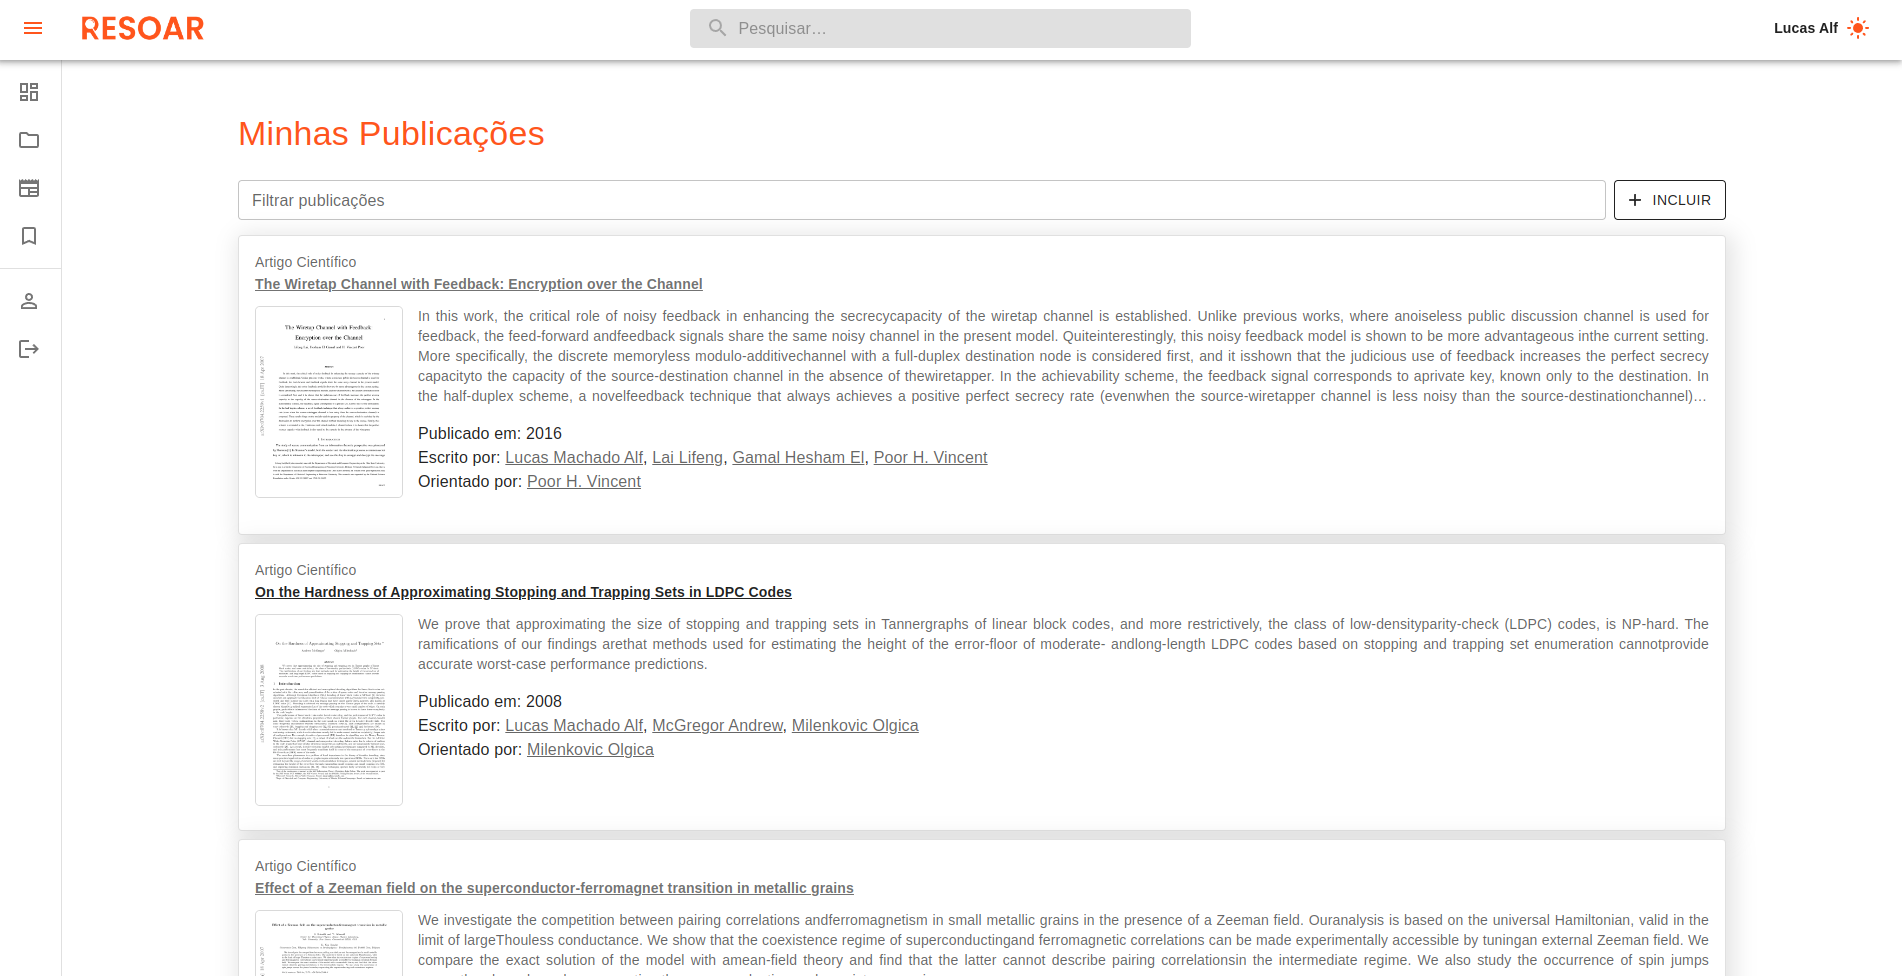
\includegraphics[scale=0.294]{img/resoar-my-research.png}}                                                                                                                                                                                                                                                                                                             \\ \hline
    \end{tabular}
\end{table}

\begin{table}[H]
    \caption{Nova publicação}
    \begin{tabular}{|p{1cm}|p{14cm}|}
        \hline
        \multicolumn{1}{|c|}{\textbf{06}} & \textbf{Nova publicação}                                                                                                                                                                                                                               \\ \hline
        \multicolumn{2}{|l|}{\begin{tabular}[c]{@{}l@{}}\textbf{Como} usuário do sistema\\ \textbf{Eu quero} realizar uma nova publicação\\ \textbf{Para que} possa salvar as minhas publicações no sistema.\end{tabular}}                                                                         \\ \hline
        \multicolumn{2}{|l|}{\textbf{Critérios de aceitação}}                                                                                                                                                                                                                                      \\ \hline
        \multicolumn{2}{|l|}{\begin{tabular}[c]{@{}l@{}}1. Deve solicitar os campos de título, resumo, ano, tipo, visibilidade, idioma,\\ instituição, autores, orientadores e arquivo da publicação.\\2. Dentro do campo de autores sempre deve haver no mínimo o próprio usuário. \end{tabular}} \\ \hline
        \multicolumn{2}{|c|}{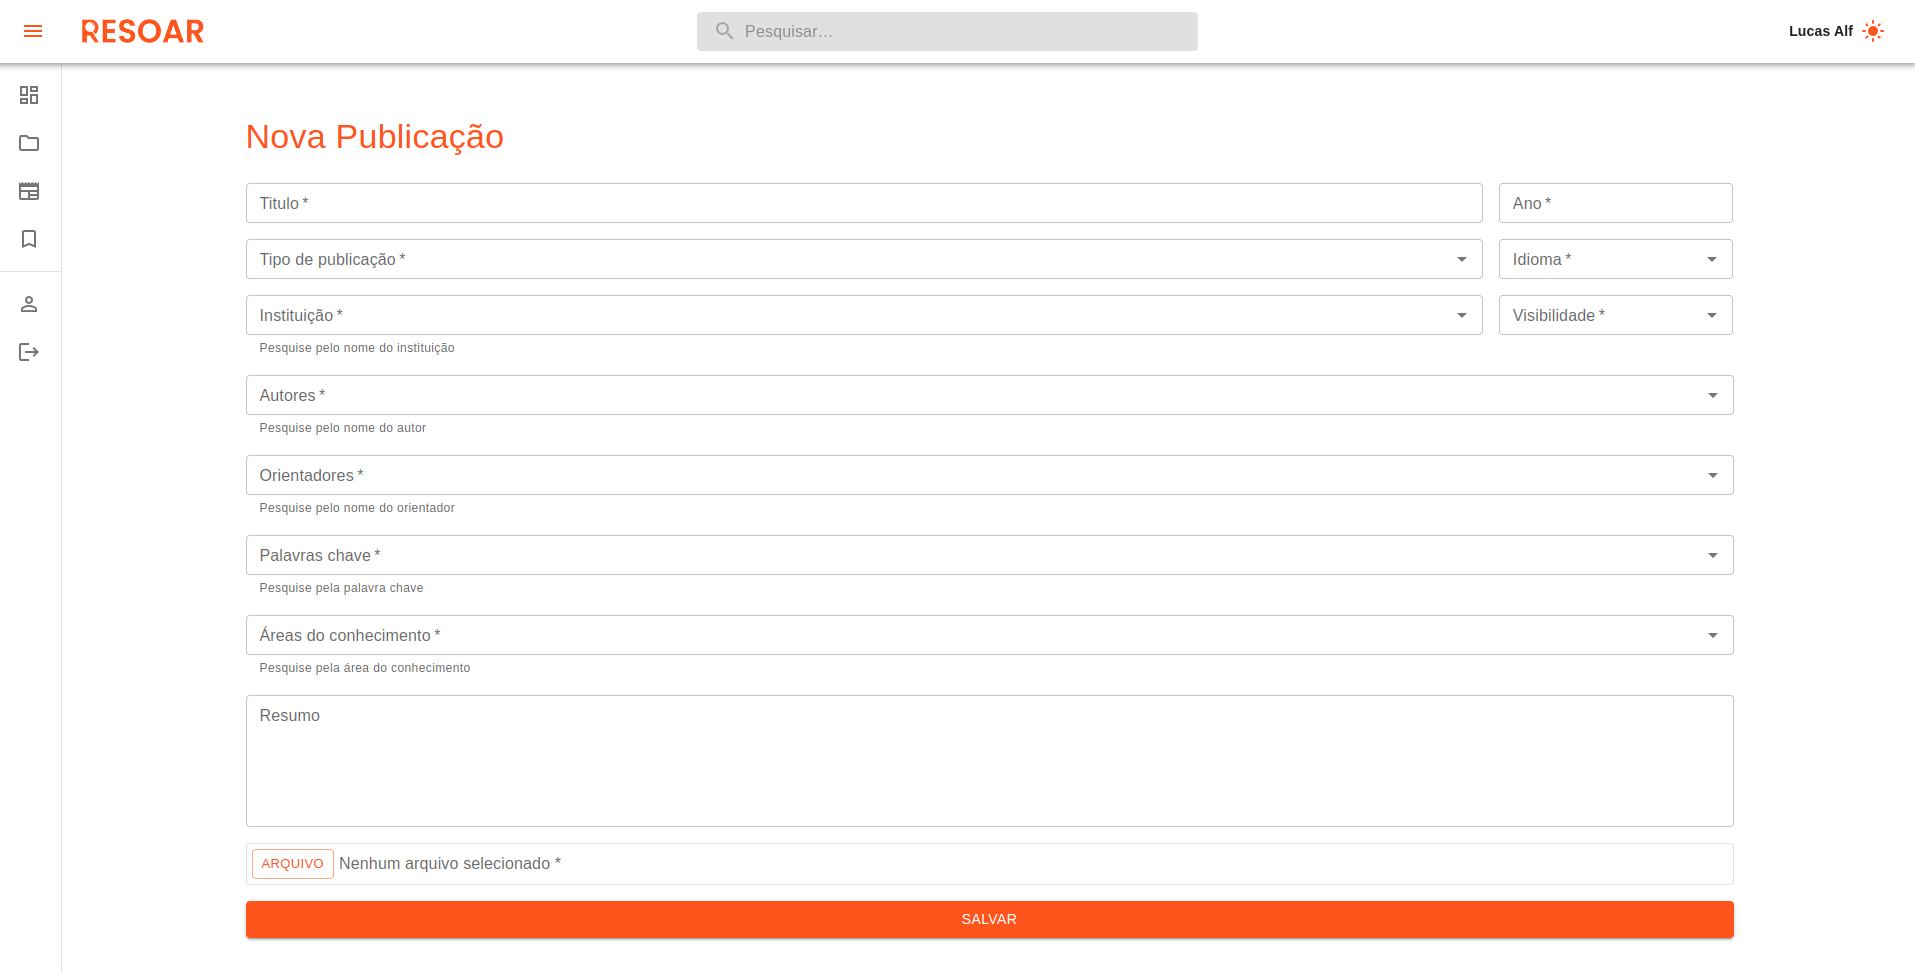
\includegraphics[scale=0.294]{img/resoar-add-research.png}}                                                                                                                                                                                                           \\ \hline
    \end{tabular}
\end{table}

\begin{table}[H]
    \caption{Pesquisar publicações}
    \begin{tabular}{|p{1cm}|p{14cm}|}
        \hline
        \multicolumn{1}{|c|}{\textbf{07}} & \textbf{Pesquisar publicações}                                                                                                                                                                                                                                           \\ \hline
        \multicolumn{2}{|l|}{\begin{tabular}[c]{@{}l@{}}\textbf{Como} usuário do sistema\\ \textbf{Eu quero} pesquisar por publicações, podendo utilizar de filtros \\ \textbf{Para que} possa encontrar as publicações que desejo visualizar.\end{tabular}}                                                         \\ \hline
        \multicolumn{2}{|l|}{\textbf{Critérios de aceitação}}                                                                                                                                                                                                                                                        \\ \hline
        \multicolumn{2}{|l|}{\begin{tabular}[c]{@{}l@{}}1. Deve permitir a busca por termos contidos dentro das publicações.\\2. Deve permitir a filtragem por ano, autor, orientador, tipo e idioma.\\3. Uma caixa de pesquisa por publicações deve estar sempre visível\\ na interface do usuário.  \end{tabular}} \\ \hline
        \multicolumn{2}{|c|}{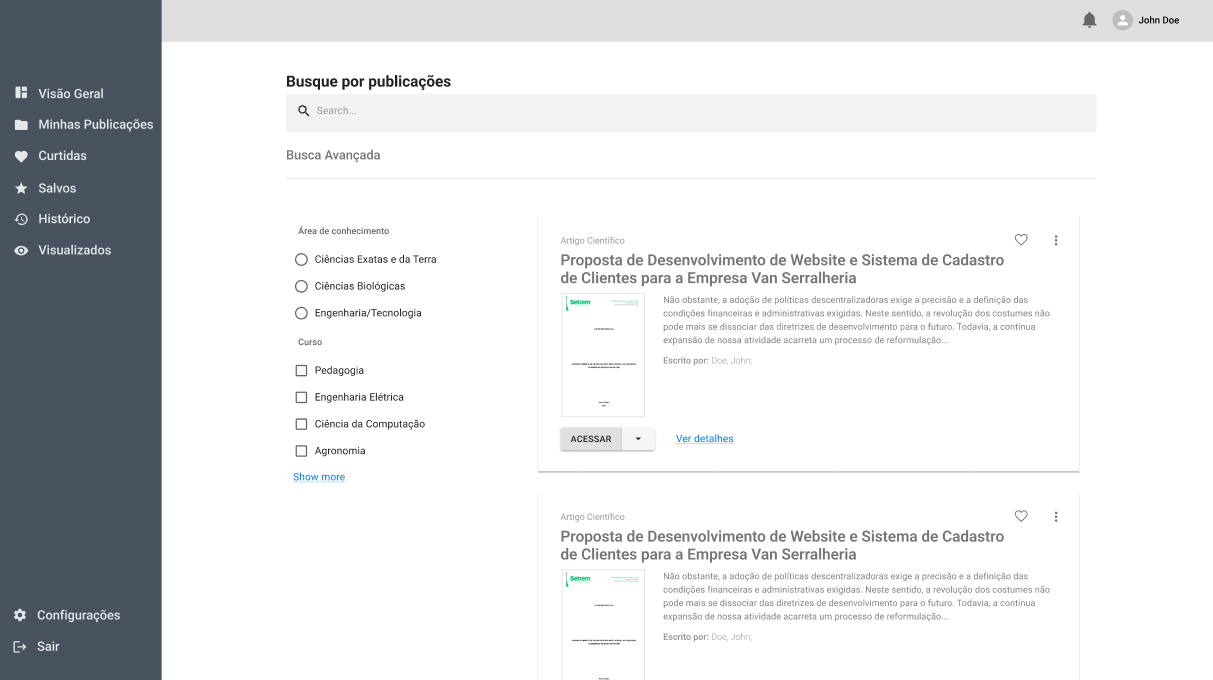
\includegraphics[scale=0.294]{img/resoar-search.png}}                                                                                                                                                                                                                                   \\ \hline
    \end{tabular}
\end{table}

\begin{table}[H]
    \caption{Detalhar publicação}
    \begin{tabular}{|p{1cm}|p{14cm}|}
        \hline
        \multicolumn{1}{|c|}{\textbf{08}} & \textbf{Detalhar publicação}                                                                                                                                                                                                                                                                                                                                                                         \\ \hline
        \multicolumn{2}{|l|}{\begin{tabular}[c]{@{}l@{}}\textbf{Como} usuário do sistema\\ \textbf{Eu quero} visualizar os detalhes de uma publicação \\ \textbf{Para que} possa ver os autores, orientadores, resumo e baixar o arquivo\\ da publicação.\end{tabular}}                                                                                                                                                                          \\ \hline
        \multicolumn{2}{|l|}{\textbf{Critérios de aceitação}}                                                                                                                                                                                                                                                                                                                                                                                    \\ \hline
        \multicolumn{2}{|l|}{\begin{tabular}[c]{@{}l@{}}1. Deve exibir o título da publicação em destaque.\\2. Deve exibir a capa da publicação, e informações como os autores,\\ orientadores, tipo de publicação, idioma e resumo.\\3. Deve permitir realizar o \emph{download} da publicação.\\4. Deve permitir salvar a publicação para mais tarde.\\5. Deve permitir gerar um \emph{link} de compartilhamento da publicação. \end{tabular}} \\ \hline
        \multicolumn{2}{|c|}{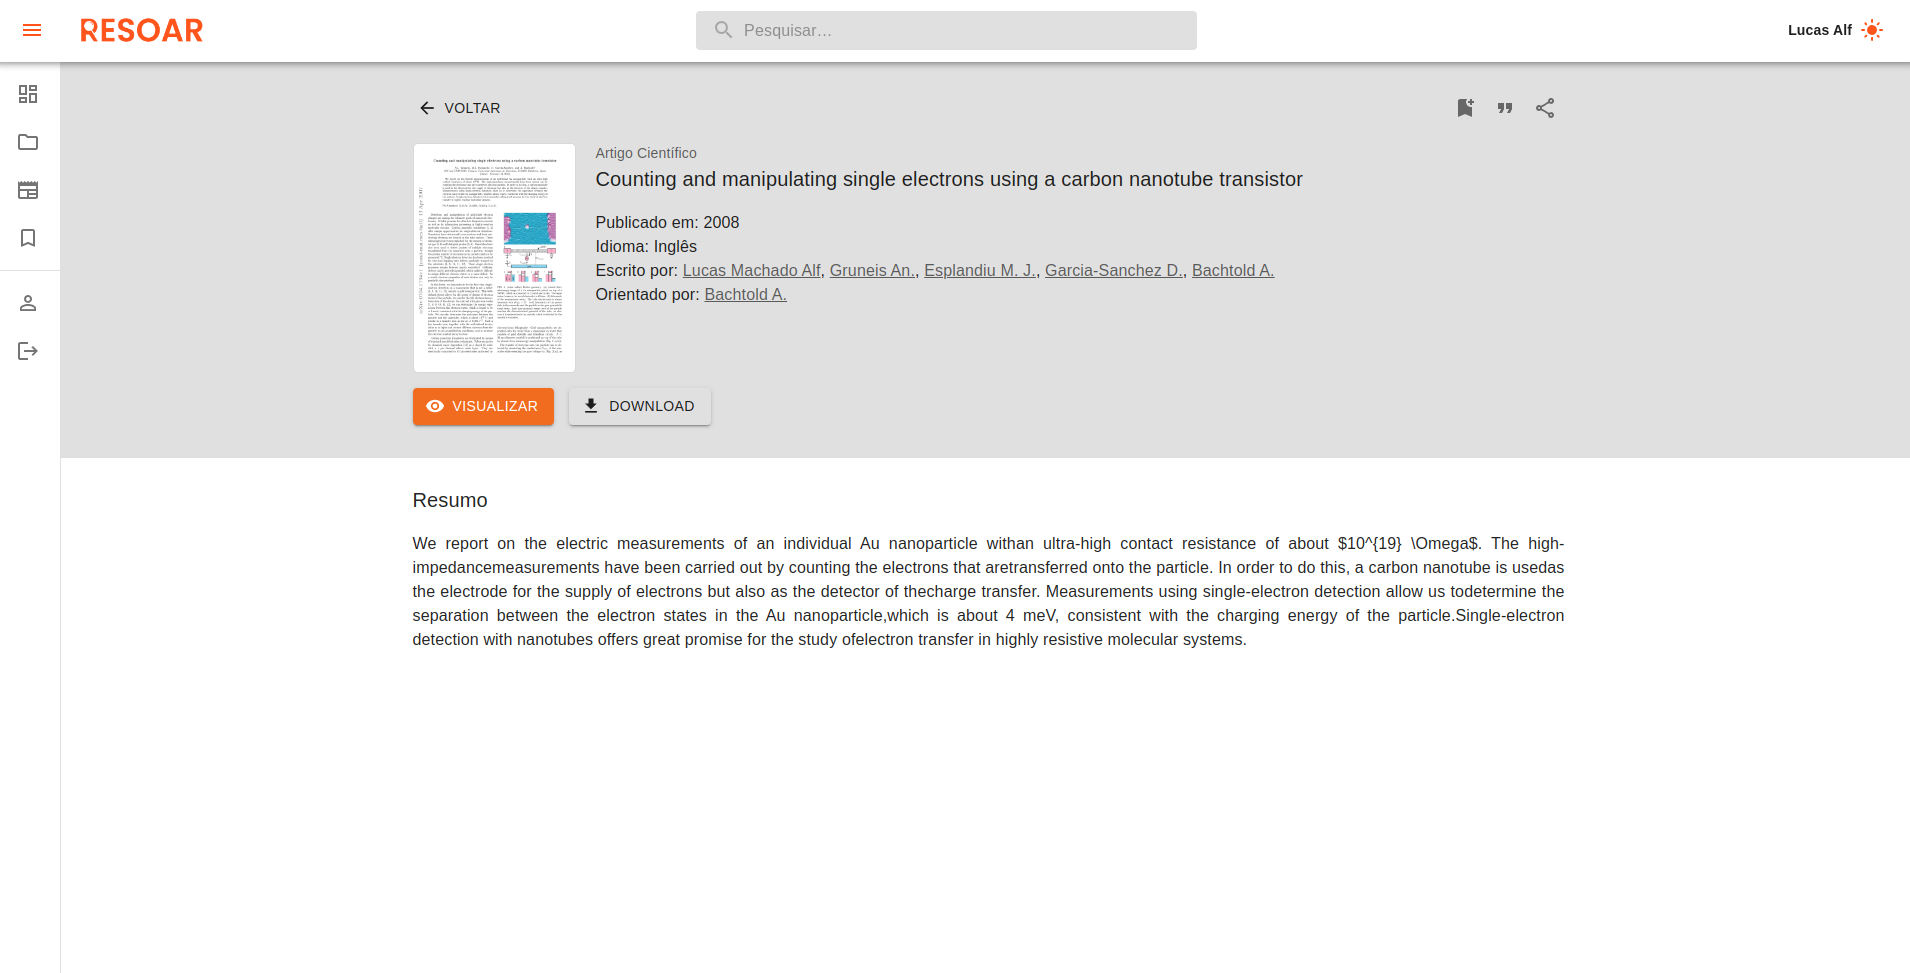
\includegraphics[scale=0.294]{img/resoar-view-research.png}}                                                                                                                                                                                                                                                                                                                                                        \\ \hline
    \end{tabular}
\end{table}

\begin{table}[H]
    \caption{Visualizar publicação}
    \begin{tabular}{|p{1cm}|p{14cm}|}
        \hline
        \multicolumn{1}{|c|}{\textbf{08}} & \textbf{Visualizar publicação}                                                                                                                                                                                                                                                   \\ \hline
        \multicolumn{2}{|l|}{\begin{tabular}[c]{@{}l@{}}\textbf{Como} usuário do sistema\\ \textbf{Eu quero} visualizar uma publicação dentro do sistema \\ \textbf{Para que} possa ver o documento sem precisar realizar o \emph{download} do arquivo.\end{tabular}}                                                        \\ \hline
        \multicolumn{2}{|l|}{\textbf{Critérios de aceitação}}                                                                                                                                                                                                                                                                \\ \hline
        \multicolumn{2}{|l|}{\begin{tabular}[c]{@{}l@{}}1. Deve permitir navegar pelas páginas do documento.\\2. Deve permitir ampliar, reduzir e rotacionar o documento.\\3. Deve permitir salvar a publicação para mais tarde. \\4. Deve permitir gerar gerar um \emph{link} para compartilhar o documento. \end{tabular}} \\ \hline
        \multicolumn{2}{|c|}{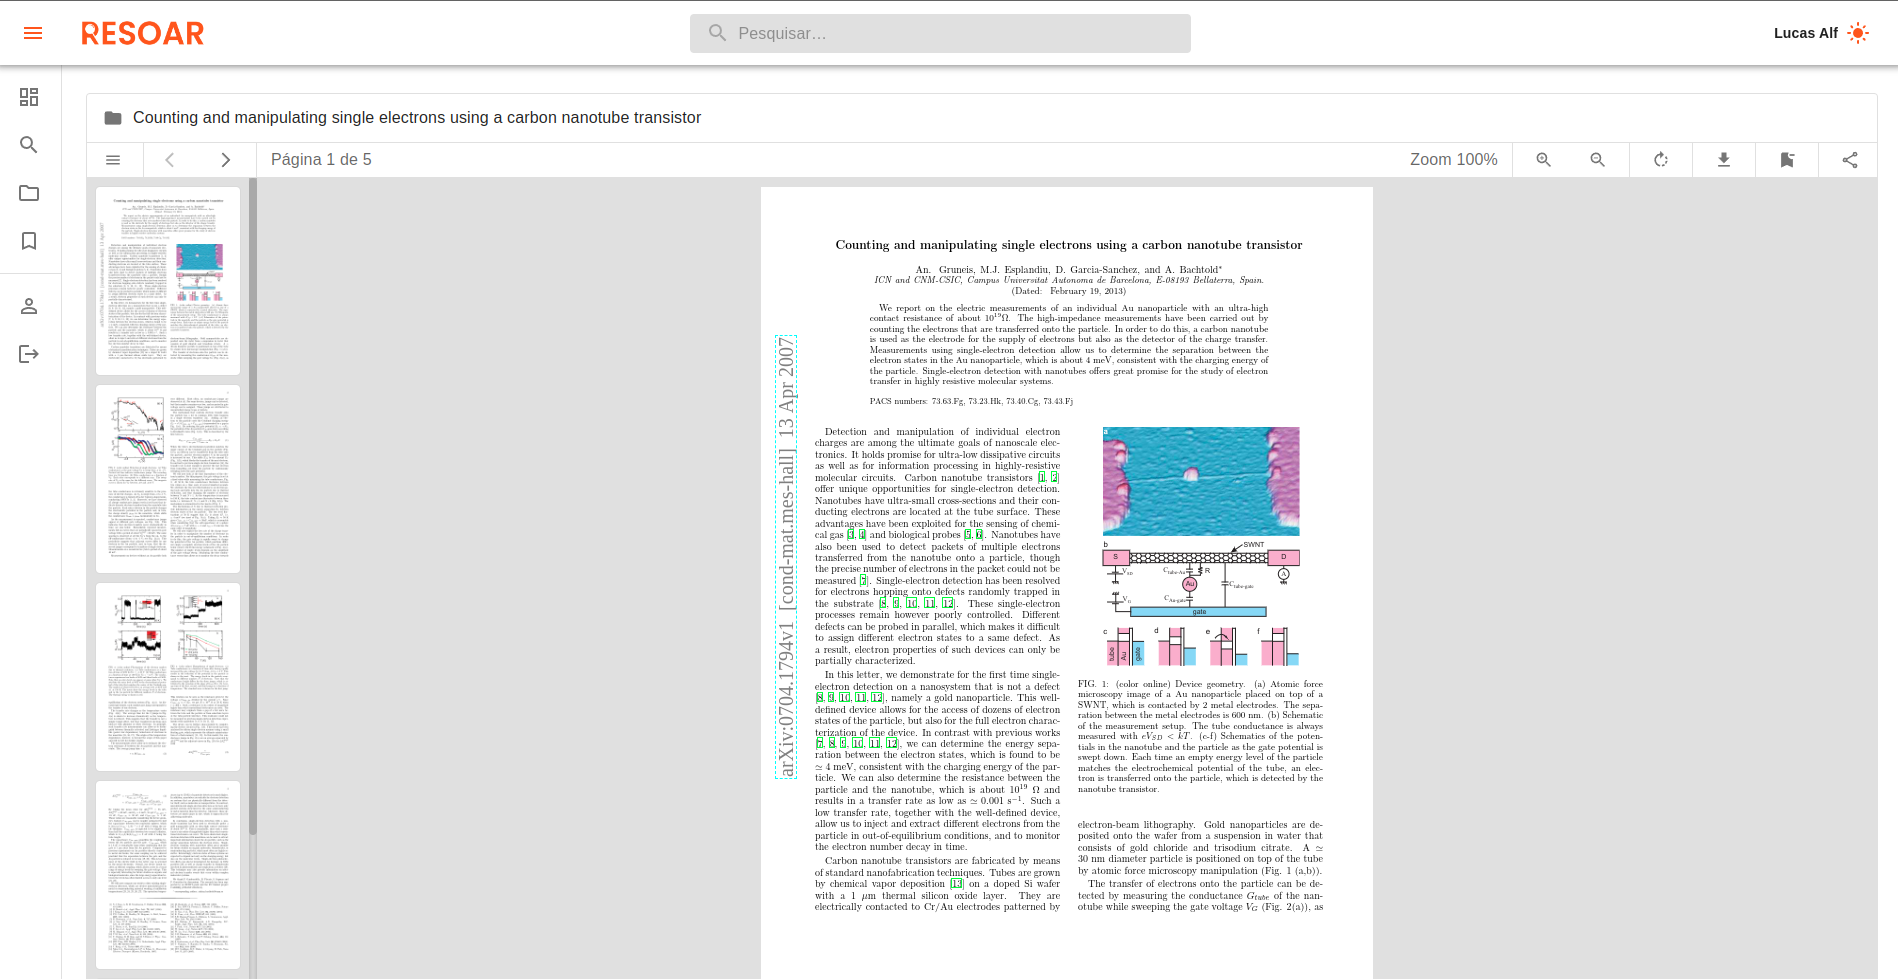
\includegraphics[scale=0.294]{img/resoar-pdf-viewer.png}}                                                                                                                                                                                                                                       \\ \hline
    \end{tabular}
\end{table}

\begin{table}[H]
    \caption{Perfil do usuário}
    \begin{tabular}{|p{1cm}|p{14cm}|}
        \hline
        \multicolumn{1}{|c|}{\textbf{09}} & \textbf{Perfil do usuário}                                                                                                                                                                                                                                                  \\ \hline
        \multicolumn{2}{|l|}{\begin{tabular}[c]{@{}l@{}}\textbf{Como} usuário do sistema\\ \textbf{Eu quero} acessar uma página de perfil de usuário \\ \textbf{Para que} possa atualizar minhas informações, e trocar minha senha.\end{tabular}}                                                                       \\ \hline
        \multicolumn{2}{|l|}{\textbf{Critérios de aceitação}}                                                                                                                                                                                                                                                           \\ \hline
        \multicolumn{2}{|l|}{\begin{tabular}[c]{@{}l@{}}1. Deve exibir o nome e a foto do usuário.\\2. Deve listar as publicações as quais o usuário participa como autor.\\3. Caso o usuário esteja acessando o seu próprio perfil, devem existir opções\\ para editar as informações e trocar a senha. \end{tabular}} \\ \hline
        \multicolumn{2}{|c|}{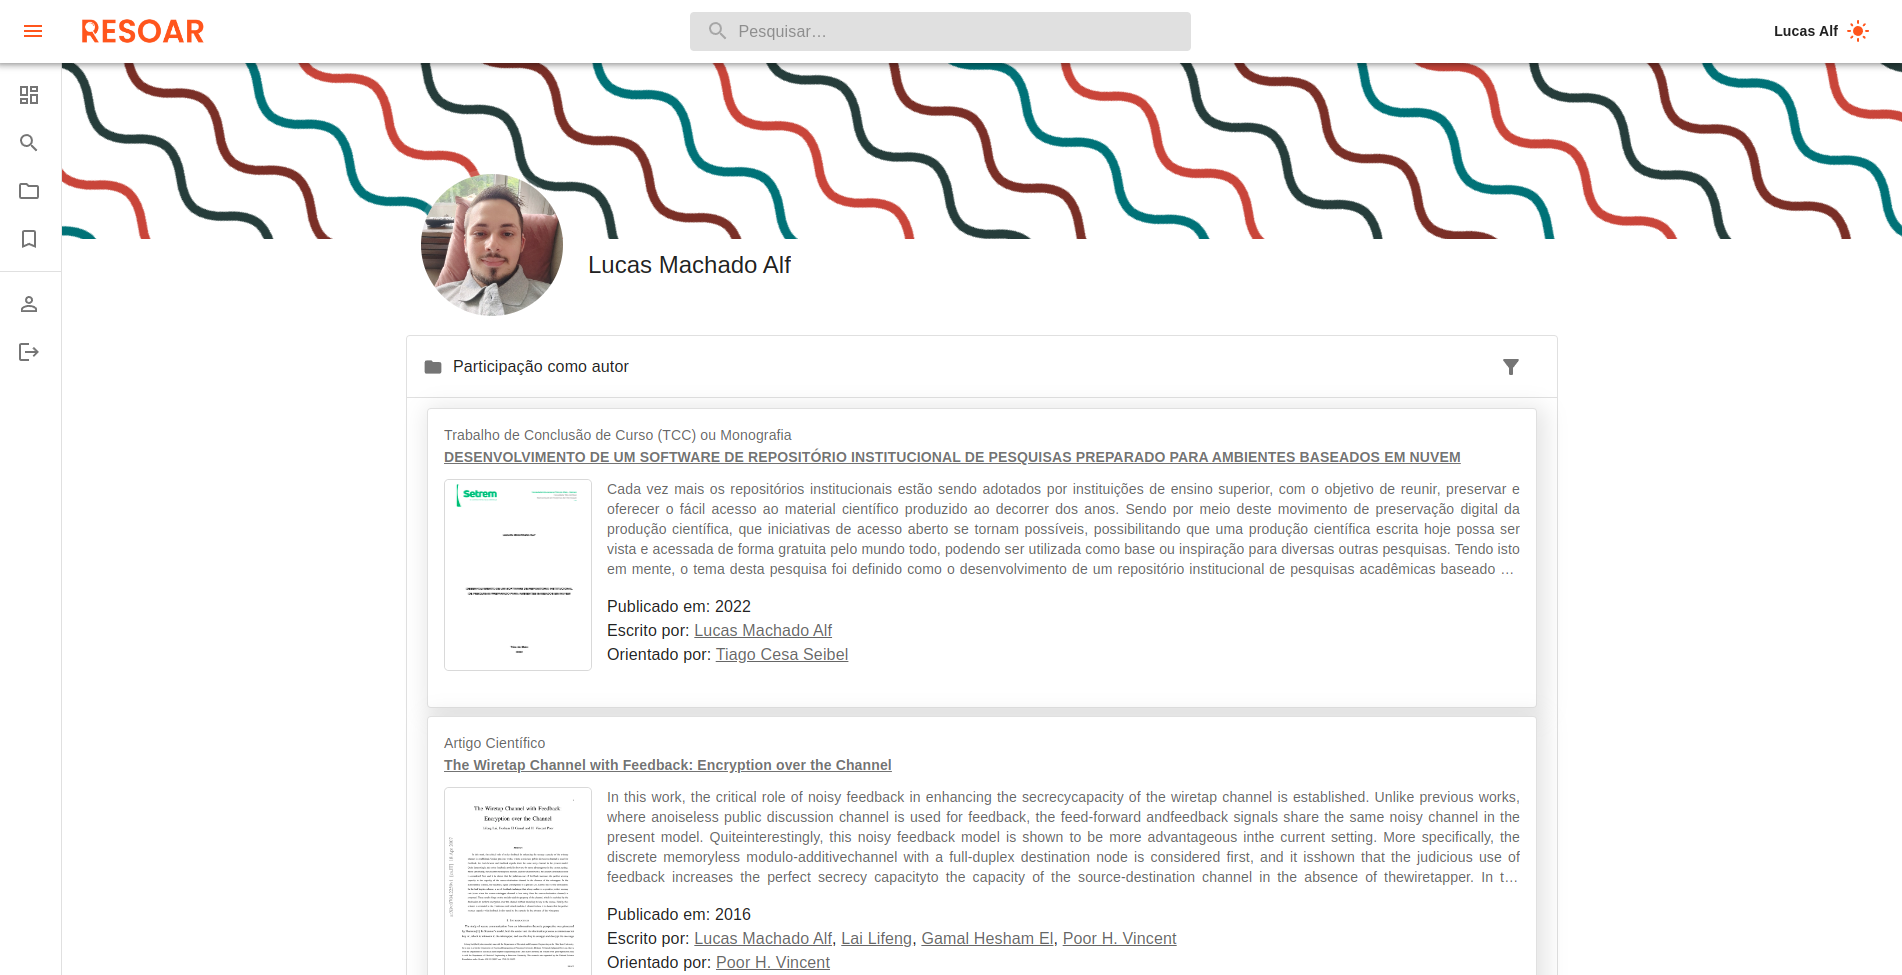
\includegraphics[scale=0.294]{img/resoar-account.png}}                                                                                                                                                                                                                                     \\ \hline
    \end{tabular}
\end{table}

\section{Arquitetura da aplicação}

Nesta seção será apresentada a estrutura utilizada para desenvolver tanto o
\emph{frontend} quanto o \emph{backend} do repositório institutional, além das
ferramentas e tecnologias utilizadas durante o processo de desenvolvimento.

Para realizar o versionamento de código, tanto do \emph{backend} quanto do
\emph{frontend} foi utilizado do GitHub\footnote{https://github.com/}, em
conjunto do SonarCloud\footnote{https://sonarcloud.io/} para a realização
de \emph{code review} automatizado, e controle de qualidade de código.

\subsection{Estrutura de Backend}

O \emph{backend} do repositório institucional consiste em uma API REST escrita na
linguagem C\#, utilizando do .NET 7. Para conexão com o banco de dados foi utilizado
do \emph{ORM} (\emph{Object Relational Mapper}) Entity Framework, porém o projeto
também oferece suporte ao \emph{Micro ORM} Dapper. Como esquema de autenticação
de usuário foi optado pelo JWT (\emph{JSON Web Tokens}).

Este projeto segue a estrutura de \emph{Repository Pattern}, em conformidade com os
conceitos do DDD (\emph{Domain-Driven Design}), que permitem a divisão do código
fonte em diversas camadas, que neste projeto foram dividas em:

\begin{enumerate}
    \item \textbf{Core}: contém as camadas de \emph{Domain} e \emph{Application},
          envolvendo as entidades que serão utilizadas para modelar o banco de dados,
          e as \emph{Services} que funcionam como uma camada intermediária, que visam
          integrar somente oque desejamos expor da camada \emph{Infrastructure} a
          camada \emph{Presentation}.

    \item \textbf{Infrastructure}: responsável por todo e qualquer acesso ou operação
          sobre o banco de dados, contendo os arquivos de configuração de conexão,
          configurações do \emph{ORM}, \emph{Migrations} e \emph{Repositories}.

    \item \textbf{Presentation}: consiste em uma API REST, responsável pela comunicação
          entre o usuário final e a aplicação, nesta camada estarão presentes as
          \emph{Controllers} e outras configurações da API.

    \item \textbf{Tests}: contém os arquivos referentes a testes unitários, testes de
          integração, ou outros \emph{scripts} de automatização de testes.
\end{enumerate}

Como banco de dados foi utilizado o PostgreSQL, visto que este possui recursos de
\emph{full-text search} embutidos, que foram utilizados para realizar a consulta
por publicações. Para realizar a modelagem do banco de dados, envés de seguir
uma estrutura tradicional de modelo ER, foi utilizado de uma abordagem
\emph{code first}, por meio do recurso de \emph{Migrations} fornecido pelo
\emph{Entity Framework}.

Para realizar o armazenamento dos arquivos das publicações, é utilizado de serviços de
\emph{Object Storage} baseados em nuvem, dando suporte ao \emph{Digital Ocean Spaces}
e ao \emph{Amazon S3}.

\subsection{Estrutura de Frontend}

O \emph{frontend} do repositório institucional foi desenvolvido majoritariamente
na linguagem de programação JavaScript utilizando do React, em conjunto do
\emph{build tool} Vite, e dos componentes visuais do Material UI.

Este projeto segue uma estrutura básica, onde os arquivo estão organizados
em pastas, que normalmente são encontradas em projetos feitos em React, sendo:
\begin{enumerate}
    \item \textbf{Assets}: contém arquivos estáticos de imagens, sons,
          arquivos de texto, etc.
    \item \textbf{Components}: contém os componentes personalizados do projeto,
          como o \emph{layout} do site, \emph{NavBar}, menu lateral, etc.
    \item \textbf{Pages}: contém as páginas do site, como a página de \emph{login},
          \emph{home}, perfil do usuário, etc.
    \item \textbf{Services}: contém os arquivos responsáveis pela comunicação
          com a API, por meio de requisições HTTP.
    \item \textbf{Themes}: contém os arquivos de estilos do projeto, como
          o tema claro, tema escuro, cores primárias, secundárias, etc.
\end{enumerate}

\section{Implantação da Aplicação}

Nesta seção será apresentado um exemplo de como o repositório institucional
desenvolvido pode ser implantado na infraestrutura de nuvem da \emph{Digital Ocean},
e como pode ser escalado para anteder altas demandas.

\subsection{Implantação em nuvem}

Para realizar a implantação do repositórios institucional em nuvem, foi escolhido
o provedor de nuvem \emph{Digital Ocean}, pois este apresentava o melhor custo-benefício
dentre os provedores de nuvem no momento que este trabalho foi realizado. Porém, é
necessário ressaltar que o sistema desenvolvido não depende exclusivamente dos
serviços oferecidos pela \emph{Digital Ocean}, podendo ser implantado em qualquer
outro provedor de nuvem, e até mesmo de forma \emph{on-premises} se necessário.

\begin{figure}[H]
    \caption{Diagrama de Infraestrutura de Nuvem}
    \centering
    \frame{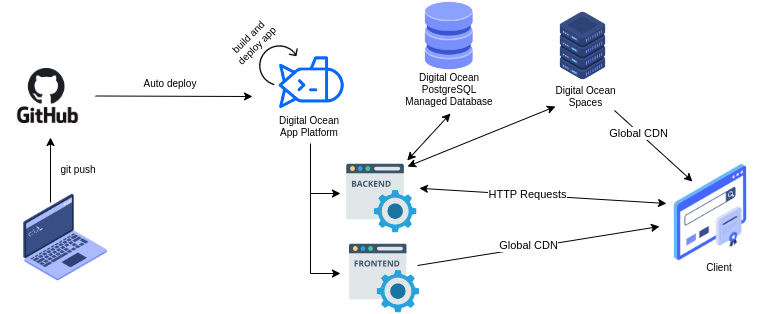
\includegraphics[scale=0.56]{img/do_infra.png}}
    \label{fig:do_infra}
\end{figure}

A Figura \ref{fig:do_infra} apresenta um modelo de como o repositório institutional
desenvolvido pode ser implantado na infraestrutura da \emph{Digital Ocean}.
No modelo apresentado, é utilizado do serviço de \emph{App Platform} oferecido pela
\emph{Digital Ocean}, para realizar a implantação do \emph{backend} e \emph{frontend}
do repositório institucional.

No \emph{App Platform} é necessário informar uma fonte para a aplicação, que neste
modelo foi utilizado do código fonte presente no \emph{GitHub}, porém poderia ser
utilizado o \emph{GitLab}, ou utilizar de imagens de container armazenadas no
\emph{Docker Hub}, ou no próprio \emph{Container Registry} oferecido pela
\emph{Digital Ocean}.

O \emph{App Platform} monitora a fonte informada, e sempre que existe uma nova versão
ele automaticamente realiza o \emph{build} da aplicação, no caso de informado o
\emph{GitHub} ou \emph{GitLab} como fonte, ou realiza o \emph{pull} da nova imagem,
caso informado o \emph{Docker Hub} ou outro \emph{Container Registry} como fonte.

O serviços implantados por meio do \emph{App Platform} podem ser facilmente escalonados
por meio do painel de controle da \emph{Digital Ocean}, tanto de forma vertical,
aumentando o número de recursos por instância, e de forma horizontal, aumentando o
número de replicas rodando de forma paralela, e distribuindo a carga por meio de um
\emph{load balancer}.

No modelo apresentado, também é utilizado de uma instância do banco de dados
\emph{PostgreSQL} por meio do serviço \emph{Managed Database}, que também
pode ser escalonado tanto de forma tanto vertical quanto horizontal por meio do painel
de controle. E o serviço de armazenamento de objetos em nuvem, denominado de
\emph{Digital Ocean Spaces}, equivalente ao serviço \emph{S3} da \emph{Amazon},
para realizar o armazenamento dos documentos. Este último em teoria não precisa
ser escalonado, visto que seus documentos já são distribuídos por meio de uma
CDN (\emph{Content Delivery Network}) global.


\section{Análise dos Resultados}

Nesta seção será apresentado os resultados dos testes realizados
sobre o repositório institucional desenvolvido, visando corroborar ou refutar
as hipóteses de desempenho da aplicação. Também serão apresentados gráficos de
métricas de utilização de processador e memória do \emph{backend} da aplicação,
visando estabelecer os requisitos mínimos do sistema.

\subsection{Preparação da base de dados}

Para a realização dos testes no repositório institucional desenvolvido,
foi realizado a preparação de uma base de dados com 3.500 publicações,
tento como base o \emph{arXiv Dataset}, que consiste em um \emph{dataset}
gratuito de publicações acadêmicas.

Para realizar a preparação da base de dados, foi realizado o \emph{download} de
3.500 publicações do \emph{arXiv Dataset} em formato PDF, e desenvolvido um algoritmo
na linguagem C\# (mesma linguagem que foi desenvolvido o \emph{backend} do repositório
institucional), que realiza a leitura do arquivo de metadados disponibilizado pelo \emph{arXiv},
e compara o identificador único presente no arquivo de metadados com os arquivos presentes
na pasta em que foi realizado o \emph{download} das publicações.

O arquivo de metadados disponibilizado pelo \emph{arXiv}, consiste em um arquivo no formato
JSON contendo uma lista de dados, como o identificador único da publicação, o nome do usuário
que publicou o artigo, o nome dos autores, o titulo da publicação, comentários, informações sobre
a revista em que o artigo foi publicado, o número DOI (\emph{Digital Object Identifier}), o resumo,
as categoriais e as revisões da publicação.

\begin{figure}[H]
    \caption{Diagrama de fluxo do algoritmo de preparação da base de dados}
    \centering
    \frame{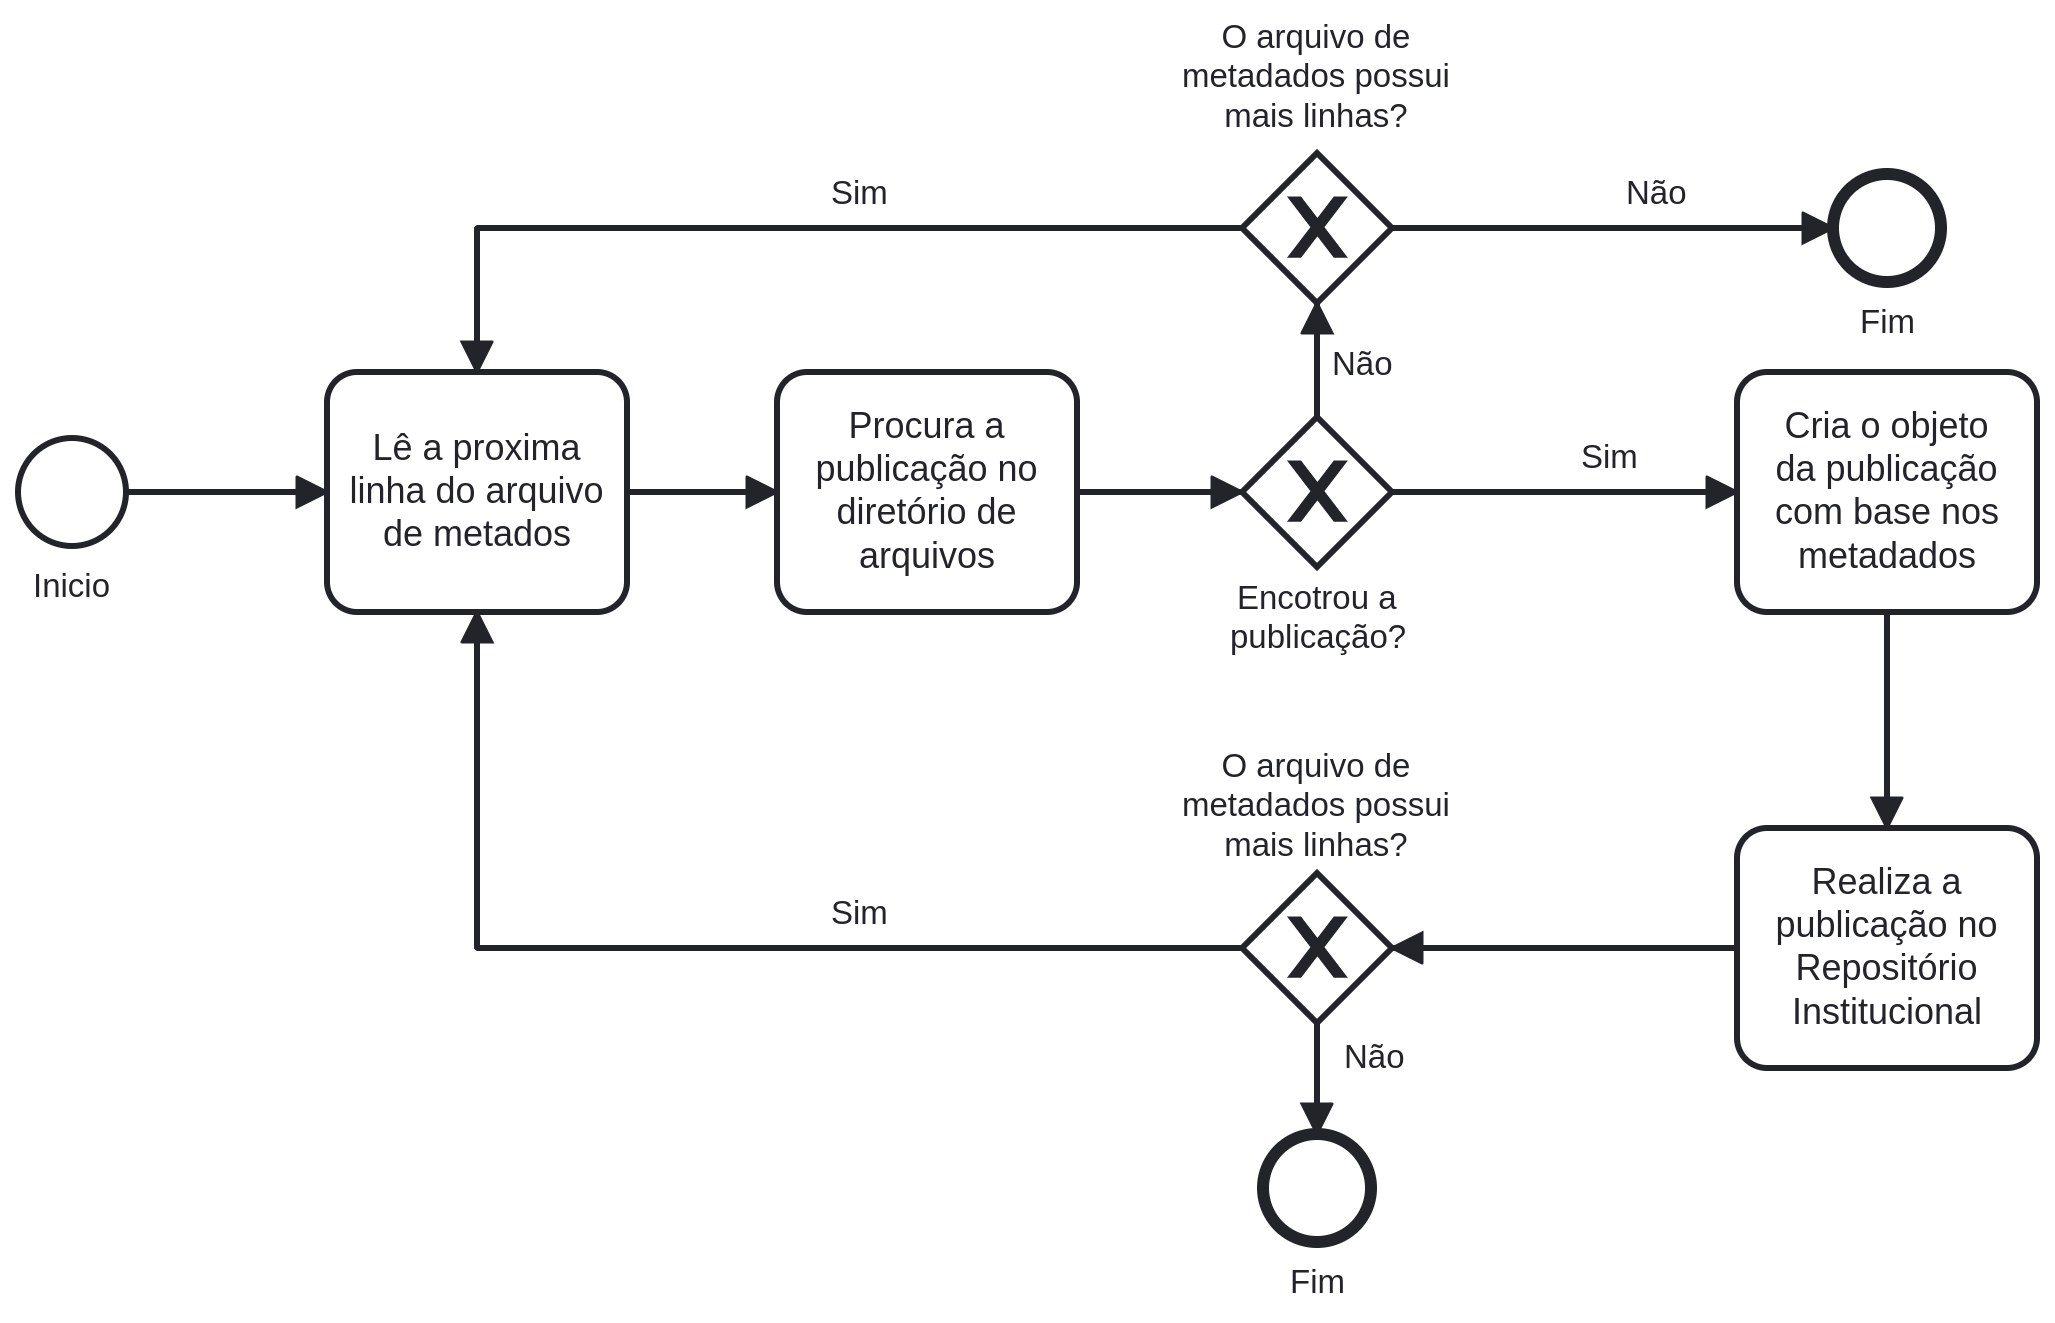
\includegraphics[scale=0.21]{img/pseudo-algoritmo.png}}
    \label{fig:pseudo-algoritmo}
\end{figure}

A Figura \ref{fig:pseudo-algoritmo} apresenta o funcionamento do algoritmo, que percorre o arquivo
de metadados, e procura pela publicação dentro da pasta onde foi realizado o \emph{download} das publicações.
O algoritmo identifica os arquivos por meio de seu nome, visto que os arquivos possuem um padrão de nomenclatura,
que consiste no identificador único concatenado ao número da revisão.

Ao encontrar uma combinação, o algoritmo realiza a transformação dos metadados do
\emph{arXiv} em um formato que o repositório institucional possa processar, e realiza
a submissão da publicação dentro do repositório institucional, passando pelo mesmo
processo que uma publicação realizada por um usuário real, porém de forma automatizada.

\subsection{Teste de Consulta por Publicações}

Para obter o tempo médio de consultas por publicações dentro do repositório
institucional, foi utilizado da ferramenta Apache JMeter, que consiste em um
\emph{software} para a realização de testes de carga e estresse.

A partir do Apache JMeter, foi preparado um cenário de teste onde uma consulta
pelo termo "\emph{Distribution of H2O}'' foi realizada por mil vezes a API do
repositório institucional. O termo utilizado na pesquisa poderia ser outro, e
foi escolhido apenas pelo conhecimento que haveria publicações com termos semelhantes
na base de dados, visto que não faria sentido realizar um teste de estresse sobre um termo
que não possuísse resultados.

\begin{figure}[H]
    \caption{Métricas de consulta por publicações}
    \frame{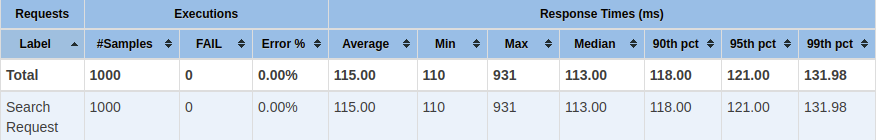
\includegraphics[scale=0.703]{img/matrics-advanced-search.png}}
    \label{fig:matrics-advanced-search}
\end{figure}

A Figura \ref{fig:matrics-advanced-search} apresenta as métricas resultantes do teste
realizado com o Apache JMeter, nesta figura é possível visualizar que houve um tempo de
resposta médio de 114,54 milissegundos por requisição, um tempo mínimo de 109,4
milissegundos, e um tempo máximo de 1131,8 milissegundos. Na figura também é possível
visualizar os valores de mediana, percentil, transações por segundo, e informações da
rede.

\begin{figure}[H]
    \caption{Tempo médio de reposta por consulta ao longo do tempo}
    \centering
    \frame{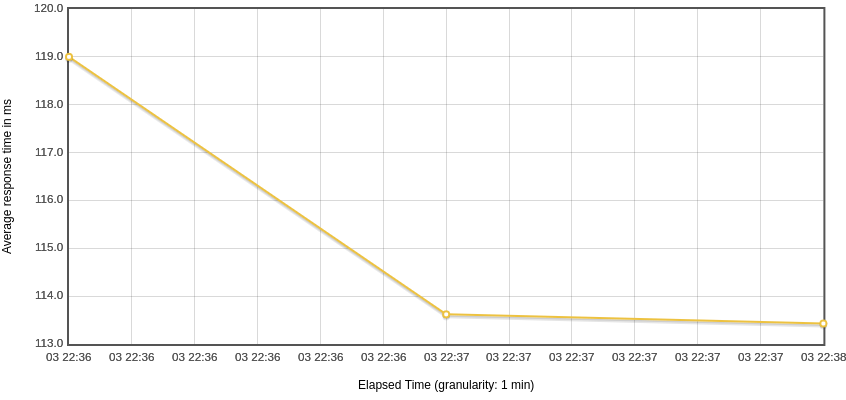
\includegraphics[scale=0.708]{img/search-response-over-time.png}}
    \label{fig:search-response-over-time}
\end{figure}

A Figura \ref{fig:search-response-over-time} apresenta o tempo médio de respostas
em milissegundos, dentro dos primeiros 31 segundos de execução do teste. Nesta figura
é possível perceber que o tempo médio de resposta diminui ao longo do tempo, iniciando
em 136,16 milissegundos, e reduzindo para valores entre 117 e 112 milissegundos ao longo
da execução. É provável que o tempo médio por consulta esteja sendo reduzido devido ao
banco de dados realizar o cache das consultas.

\begin{figure}[H]
    \caption{Uso de recursos do \emph{backend} por consulta ao longo do tempo}
    \centering
    \frame{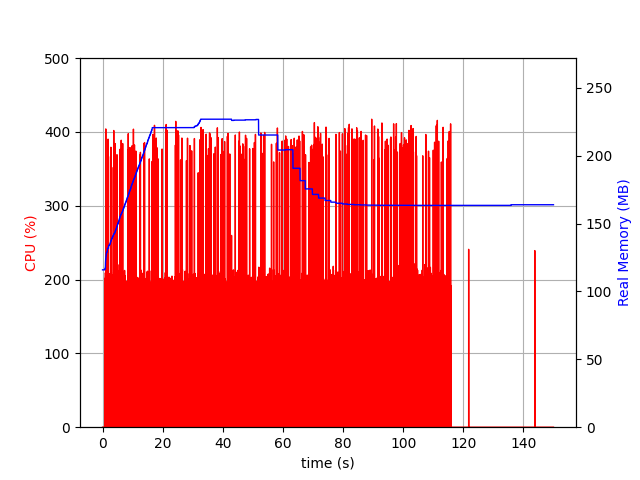
\includegraphics[scale=0.85]{img/resource-usage-advanced-search.png}}
    \label{fig:resource-usage-advanced-search}
\end{figure}

A Figura \ref{fig:resource-usage-advanced-search} apresenta o uso de recursos
de memória e processador do \emph{backend} do repositório institucional ao longo
dos primeiros 150 segundos de execução do teste. Estas métricas foram coletadas por
meio da ferramenta \emph{psrecord}\footnote{https://github.com/astrofrog/psrecord}.

Nesta mesma figura é possível visualizar que durante o teste ouve um pico de 559,62 MB
de utilização de memória, minima de 198,73 MB, e média de 471,09 MB. Já a utilização de
processador teve picos acima de 400\% visto que o teste foi executado em um
processador com quatro núcleos, porém em grande parte do tempo se manteve acima de 200\%,
demonstrando que o \emph{backend} está aproveitando os múltiplos núcleos do processador.

\subsection{Teste de Submissão de Publicações}

Da mesma forma que o teste de consulta por publicações, o teste de submissão de
publicações também foi elaborado a partir do Apache JMeter. Para obter o tempo médio
de submissão de publicação, foi preparado um cenário de teste onde uma mesma publicação
com 12.000 palavras (cerca de 40 páginas de texto em português com fonte tamanho 12,
considerando que cada página tenha 300 palavras) foi realizada por mil vezes a API do
repositório institucional.

\begin{figure}[H]
    \caption{Métricas de submissão de publicações}
    \frame{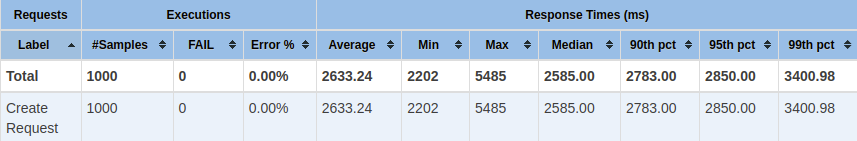
\includegraphics[scale=0.703]{img/matrics-create-research.png}}
    \label{fig:matrics-create-research}
\end{figure}

A Figura \ref{fig:matrics-create-research} apresenta as métricas obtidas através do
teste, onde é possível visualizar que houve um tempo médio de resposta de 2,56 segundos,
com um tempo mínimo de 2,30 segundos, e um tempo máximo de 6,62 segundos. A figura também
apresenta os valores de mediana, percentil, transações por segundo, e informações de rede.

\begin{figure}[H]
    \caption{Tempo médio de reposta por submissão ao longo do tempo}
    \centering
    \frame{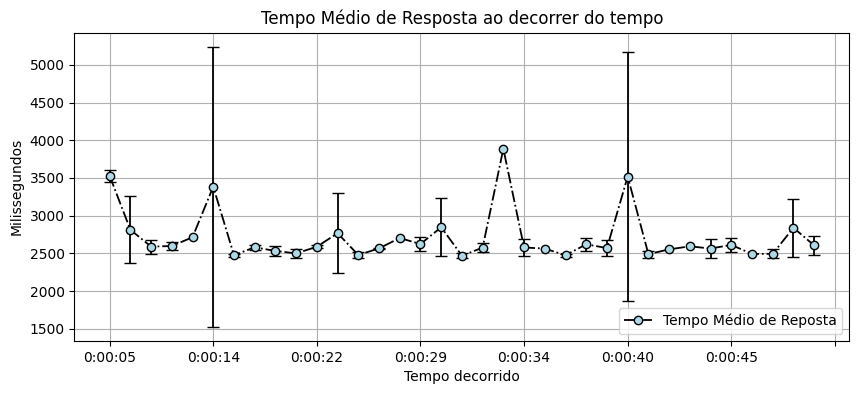
\includegraphics[scale=0.70]{img/create-response-over-time.png}}
    \label{fig:create-response-over-time}
\end{figure}

A Figura \ref{fig:create-response-over-time} apresenta o tempo médio de resposta
de submissão de publicação ao longo dos primeiros 50 segundos do teste, onde é
possível visualizar que as primeiras publicações realizadas levam em média
3,52 segundos para serem concluídas, e este tempo logo em seguida é reduzido, e se
mantém entre 2,5 e 2,8 segundos.

\begin{figure}[H]
    \caption{Uso de recursos do \emph{backend} por submissão ao longo do tempo}
    \centering
    \frame{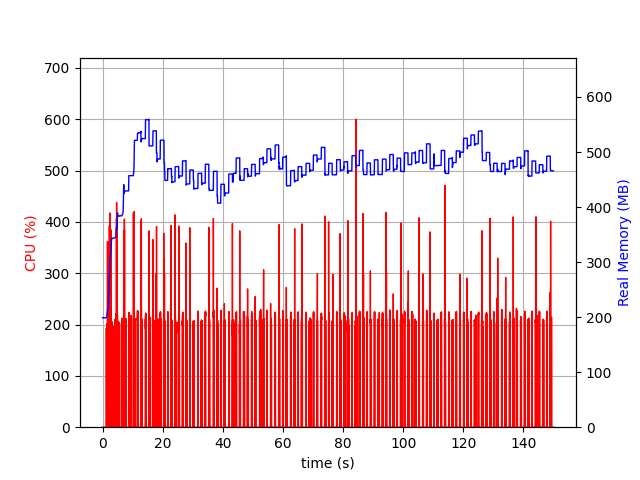
\includegraphics[scale=0.93]{img/resource-usage-create-research.png}}
    \label{fig:resource-usage-create-research}
\end{figure}

Já a Figura \ref{fig:resource-usage-create-research} demonstra o uso de recursos
de memória e processor do \emph{backend} do repositório institucional, ao longo
dos primeiros 150 segundos da execução do teste de submissão de publicações.
Da mesma forma que o gráfico de uso de recurso por consultas, estas métricas
também foram coletadas por meio da ferramenta \emph{psrecord}.

Nesta mesma figura é possível visualizar que durante a execução do teste houve uma
utilização máxima de 559,62 MB de memória, minima de 198,73 MB, e média de 471,09 MB.
Também é perceptível que a curva de utilização de memória parece um pouco quadriculada,
isso ocorre devido ao tempo necessário para realizar o \emph{upload} do arquivo PDF
aos servidores da Digital Ocean, que é o \emph{Cloud Provider} utilizado para o
armazenamento das publicações.

O gráfico também demonstra que o \emph{backend} do repositório institucional
está aproveitando dos múltiplos núcleos do processador para processar as requisições,
porém na maior parte do tempo a carga parece estar sendo dividida em dois núcleos.

\subsection{Requisitos Mínimos do Sistema}

Com base nas métricas coletadas através dos testes de carga e estresse apresentados
no tópico anterior, foram definidos os requisitos mínimos de \emph{hardware}
para realizar a execução do repositório institucional desenvolvido.

\subsubsection{Frontend}

Por se tratar de um site estático desenvolvido em React, o \emph{frontend} desenvolvido
para o repositório institucional não possui requisitos mínimos de CPU ou memória, podendo
ser hospedado em qualquer provedor de nuvem que ofereça a opção de hospedagem de sites
estáticos, realizando o cache dos arquivos em CDN (\emph{Content Delivery Network}).

Alguns provedores de nuvem fornecem a opção de realizar este tipo de hospedagem forma
gratuita, em conjunto com HTTPS também gratuito, como no caso da Digital Ocean App Platform\footnote{https://www.digitalocean.com/products/app-platform}
e do Vercel\footnote{https://vercel.com/}.

Já no quesito de compatibilidade com navegadores, o \emph{frontend} desenvolvido segue
os mesmos padrões de compatibilidade do Vite 3, necessitando de suporte a \emph{JavaScript}
moderno, módulos \emph{JavaScript} nativos, importação dinâmica de módulos nativos,
e suporte ao \textbf{import.meta}.

\begin{enumerate}
    \item \textbf{Chrome} >= 87
    \item \textbf{Firefox} >= 78
    \item \textbf{Safari} >= 13
    \item \textbf{Edge} >= 88
\end{enumerate}

O suporte a navegadores legados poderia ser implementado por meio de
tecnologias como o Polyfill\footnote{https://polyfill.io}, porém foi
optado por oferecer suporte por padrão somente a navegadores modernos.

\subsubsection{Backend}

Com base nos dados coletados durantes os testes de carga e estresse,
e nos requisitos do .NET 7, foram elaborados dois conjuntos de requisitos
para a execução do \emph{backend} do repositório institucional, sendo os
requisitos mínimos, e os recomendados.

\begin{table}[H]
    \caption{Requisitos mínimos de \emph{backend}}
    \label{quad:requisitos-backend}
    \begin{tabular}{|p{9.5cm}|ll|}
        \hline
        \textbf{Recurso}    & \multicolumn{1}{l|}{\textbf{Mínimo}}        & \textbf{Recomendado} \\ \hline
        CPU                 & \multicolumn{1}{l|}{1 vCPU}                 & 2 vCPU+              \\ \hline
        Memória RAM         & \multicolumn{1}{l|}{512 MB}                 & 1 GB+                \\ \hline
        Armazenamento       & \multicolumn{1}{l|}{4.5 GB}                 & 4.5 GB+              \\ \hline
        \multirow{3}{*}{OS} & \multicolumn{2}{l|}{Debian 10+ x64}                                \\ \cline{2-3}
                            & \multicolumn{2}{l|}{Ubuntu 18.04+ x64}                             \\ \cline{2-3}
                            & \multicolumn{2}{l|}{Alpine Linux 3.15+ x64}                        \\ \hline
    \end{tabular}
\end{table}

O Quadro \ref{quad:requisitos-backend} apresenta os requisitos mínimos e recomendados de
CPU, memória RAM, armazenamento e sistema operacional. Devido ao uso de algumas bibliotecas
como o \emph{SkiaSharp} para a manipulação de imagens, o \emph{backend} somente possui
suporte a sistemas operacionais Linux.

Também é necessário ressaltar que os requisitos mínimos apenas devem ser utilizados
em ambientes de testes. Em ambientes de produção com usuários ativos utilizado
o sistema, deve ser utilizado de requisitos iguais ou superiores aos recomendados.

\subsubsection{Banco de dados}

Como requisito de banco de dados, deve ser utilizado do PostgreSQL 14 ou superior,
já os requisitos de \emph{hardware} variam de acordo com o número de usuários ativos
utilizando o sistema.

\begin{table}[H]
    \caption{Requisitos de banco de dados}
    \label{quad:requisitos-database}
    \begin{tabular}{|p{9.7cm}|c|c|}
        \hline
        {\textbf{Recurso}} & {\textbf{Mínimo}} & {\textbf{Recomendado}} \\ \hline
        {CPU}              & {1 vCPU}          & {2 vCPU+ }             \\ \hline
        {Memória RAM}      & {1 GB}            & {4 GB+ }               \\ \hline
        {Armazenamento}    & {10 GB}           & {25 GB+ }              \\ \hline
    \end{tabular}
\end{table}

O Quadro \ref{quad:requisitos-database} apresenta os requisitos de \emph{hardware}
mínimos e recomendados para o banco de dados do repositório institucional.
Os requisitos mínimos devem ser utilizados somente em ambientes de testes,
onde existam ao máximo 22 conexões simultâneas ao banco de dados.

Em ambientes de produção, deve ser utilizado de requisitos iguais ou superiores
aos recomendados, também sendo indicado a utilização de um sistema de \emph{pool}
de conexões como o \emph{pgBouncer}\footnote{https://www.pgbouncer.org/}
para melhores resultados.

